\chapter{Theoretical Background} \label{sec:theory}
The current section will begin with definitions of terms used throughout the thesis. Then, an introduction to some key areas of \ac{ml} and \ac{dl} will be given alongside a short overview of state-of-the-art \ac{dl} methods. Finally, the principle functionality of a jet engine will be described, followed by an explanation of damage in the context of the certified service life of an engine.

\section{Definitions}
The notation \(i \in \left[m, n\right]\) is used to denote a finite set of consecutive integer values \(i\) with \(m \leq i \leq n\), where \(i,\,m,\,n \in \mathbb{N}\), i.e.
\begin{align}
    i = \left[m,\,m+1,\,m+2,\,\ldots,\,n-2,\,n-1,\,n\right].
\end{align}
Individual values are represented by lower-case letters, e.g. \(y\), while their upper-case counterparts \(Y\) represent a collection of values in two or more dimensions.

A \textbf{\ac{uts}} \(X\) of length \(l\) is a sequential collection of values \(x_{i}\) given by
\begin{align}
    X = \left[x_{1},\,x_{2},\,\ldots,\,x_{l}\right]
\end{align}
where \(x_{i} \in \mathbb{R}\) with \(i \in \left[1, l\right]\).

An \(m\)-dimensional \textbf{\ac{mts}} \(X\) of length \(l\) is a collection of \(m\) time series of length \(l\). Each of the \(m\) dimensions of the \ac{mts} can also be called a channel.
\cite[]{ismail_fawaz_deep_2019}

In the practical part of this thesis, a \textbf{dataset} \(D\) of length \(n\) is a set of \(n\) pairs of input data \(X_i\) and corresponding output data \(Y_i\), i.e.:
\begin{align}
    D = \left\{\left(X_1,\,Y_1\right), \left(X_2,\,Y_2\right), \ldots, \left(X_n,\,Y_n\right)\right\}
\end{align}
where for all \(i \in \left[1, n\right]\), \(X_i\) is a univariate or multivariate time series, and \(Y_i\) contains the given output values corresponding to \(X_i\).

A \textbf{sample} is a single pair \(\left(X_i,\,Y_i\right)\) for some \(i \in \left[1, l\right]\), and \(i\) is referred to as its \textbf{index}.

In a classification task, for some sample with index \(i\), \(Y_i\) will have length \(k\) where \(k\) is the number of possible classes that could be attributed to \(X_i\). Additionally, all \(Y_{i,j} = 0\) for each class index \(j \in \left[1, k\right]\) except where \(j\) is given as the class of \(X_i\), in which case \(Y_{i,j} = 1\).

In a regression task, \(Y_i\) has length \(k\) where \(k\) is the number of output values desired and each \(Y_{i,j} \in \mathbb{R}\) for \(j \in \left[1, k\right]\).

\section{Big Data}
The term \textit{Big Data} describes enormous datasets have become the norm over the past two decades due to the ubiquity of data-collecting devices and their increasing connectivity. It covers datasets of such great size that new methods are required to organise and extract useful information from them, as the data is often unstructured and noisy \cite[]{fan_mining_2013,chen_big_2014}.

One increasingly important, as well as highly challenging \cite[]{yang_10_2006}, data type is that of time series. A time series is a set of values ordered chronologically. It is often used in analyses for detecting trends and making predictions (on financial data, for example \cite[]{krollner_financial_2010}), but, within a \ac{ml} context, has in recent years been used for classification \cite[]{dau_ucr_2019,ismail_fawaz_deep_2019} and, in this thesis, regression.

\section{Machine Learning}
The desire to extract value from such datasets has led to an enormous increase in the popularity of machine learning (ML).

\ac{ml} is a subfield of \ac{ai}, the field of research that occupies itself with giving machines the ability to think and learn. In \ac{ml}, machines attempt to extract information and patterns from data without thorough or explicit instructions, often making use of highly contrived data. Classifying objects based on a finite set of selected input values (e.g. birds based on their weight, wingspan, the colour of their back and whether they have webbed feet \cite[]{harrington_machine_2012}) is a task for which machine learning is regularly used.

\ac{ml} tasks are generally split into two categories: supervised and unsupervised learning. The former involves training a model to associate input data with known output data in order to use the model on previously unseen data; in the latter, a model is given data and instructed to find patterns or groups based on input data alone \cite[]{goodfellow_deep_2016,kelleher_fundamentals_2015}.

\subsection{Polynomial Regression} \label{sec:polyreg}
Although regression analysis has its roots in statistics, it has great overlaps with \ac{ml} due to its root objective: to map a number of inputs (the independent variables \(x_1,\,x_2,\,\ldots,\,x_n\)) to a given continuous output (the dependent variables \(y_1,\,y_2,\,\ldots,\,y_n\)), and to predict outputs for previously unseen input data. Since the dependent variable data is known in the training data, regression analysis is a type of supervised machine learning.

A (\(n\)-dimensional) linear regression maps a linear model
\begin{align}
    y = a_0 + a_1 x_1 + a_2 x_2 + \ldots + a_n x_n
\end{align}
to given data and attempts to find the parameters \(a_i\), \(i \in \left[0, n\right]\) that provide the best fit. In the Python library \texttt{scikit-learn} \cite[]{scikit-learn}, the \texttt{LinearRegression} class\footnote{\url{https://scikit-learn.org/stable/modules/generated/sklearn.linear_model.LinearRegression.html}} determines these by minimising the residual sum of squares between the given samples and the values predicted by the fitted model.

For non-linear relationships, each \(x_i\) can be transformed using some basis function \(g_i\) after which the coefficients \(a_i\) can be determined in the same way as in the linear case. A polynomial regression is carried out by defining the basis function as \(g(x_i) = x^i\), leading to the polynomial function
\begin{align}
    f(x) = y = a_0 + a_1 x + a_2 x^2 + \ldots + a_n x^n.
\end{align}
It should be noted that, although the function is now polynomial, the model is still linear since the basis function only serves to transform the input data to a higher dimension; after the transformation using \texttt{scikit-learn}'s \texttt{PolynomialFeatures} class, the \texttt{LinearRegression} class will determine the coefficients \(a_1,\,\ldots,\,a_n\) as before.

The performance of a regression is usually measured using the coefficient of determination, \(R^2\), which compares the predicted output values to the mean of the expected output data \(\bar{y}\), and is given by
\begin{align}
    R^2 = 1 - \frac{SS_{\text{res}}}{SS_{\text{tot}}}
\end{align}
where
\begin{align}
    SS_{\text{res}} = \sum_{i=1}^{n}{\left(y_i - f(x_i)\right)}^2
\end{align}
is the residual sum of squares, and
\begin{align}
    SS_{\text{tot}} = \sum_{i=1}^{n}{\left(y_i - \bar{y}\right)}^2
\end{align}
is the total sum of squares. According to this measure, a perfect fit is indicated by a performance of \(R^2 = 1\), a fit that is no better than the mean of the output data by \(R^2 = 0\), and a fit that is even worse than the mean by \(R^2 < 0\).

\section{Deep Learning}
\ac{dl} is an application of \ac{ml} that employs more complex models capable of making sense of noisier, largely unprocessed data, such as sound signals and images \cite[]{goodfellow_deep_2016}. A bird classification problem could in this case involve training a model to extract necessary information from an image of a bird and associating this with the bird's label, requiring only the correct labelling of the image with no manual measurements.

The great advantage of \ac{dl} over \ac{ml} is its ability to make sense of complex data using simpler representations in a hierarchical system \cite[]{goodfellow_deep_2016}. Returning to the example of bird classification: To extract information on a bird from a photo, a trained model might analyse an input image for contours and corners; in the next layer, these could be combined to recognise edges, which a subsequent layer could recognise as beaks or wings, and so on. To reach this stage, however, the architecture of the model must be suitable and the model itself must be trained using enough input data of sufficient quality. To achieve an acceptable level of accuracy, models should be trained on roughly 5\,000 samples per class, with several orders of magnitude more required to achieve human-level accuracy \cite[p. 20]{goodfellow_deep_2016}.

\ac{dl} has seen a huge rise in popularity in recent years, with applications including speech recognition \cite[]{deng_machine_2013}, medical diagnoses \cite[]{lee_diagnosis_2018}, stock market prediction \cite[]{krollner_financial_2010} and many others \cite[]{kelleher_fundamentals_2015}. One particular challenge among the \ac{dl} research community is time series data \cite[]{yang_10_2006}, a sequential collection of values recorded over time. Time series data remains a great challenge due to its noisy, multidimensional nature \cite[]{kelleher_fundamentals_2015} and the dfficulties involved in developing algorithms that can also interpret the temporal information it holds \cite[]{bagnall_great_2017}.

\subsection{Neural Networks}
Two types of neural networks are relevant to this thesis: the \ac{mlp} and the \ac{cnn}. The fundamental element of the both of these is the perceptron.

\paragraph*{Perceptron}
The perceptron is a simple mathematical function somewhat inspired by biological neurons \cite{rosenblatt_perceptron_1958}. A perceptron (Figure \ref{fig:perceptron}) takes the sum of \(n\) values \(x_{1},\,x_{2},\,\ldots,\,x_{n}\) multiplied with their respective weights \(w_{1},\,w_{2},\,\ldots,\,w_{n}\) as its input. This input value is added to the perceptron's bias \(b\) and fed into its activation function \(f\). The result of this function is the perceptron's output value \(z\) which is fed into the next layer of the network. This is described by the following formula:
\begin{align}
    z = f\left(b + \sum_{i = 1}^{n}x_{i}w_{i}\right)
\end{align}
\begin{figure}
    \centering
    \begin{tikzpicture}
        \node[functions] (center) {};

        \node[below=0em of center, font=\scriptsize, text width=3em] {Activation function};
        \draw[thick] (0.6em,0.6em) -- (0,0em) -- (-0.75em,0em);
        \draw (0em,0.75em) -- (0em,-0.75em);
        \draw (0.75em,0em) -- (-0.75em,0em);
        \node[right=2em of center] (right) {};
            \path[draw,->] (center) -- (right);

        \node[functions,left=2em of center,minimum size=4em] (left) {\(b,\, \sum\)};
            \path[draw,->] (left) -- (center);
        \node[weights,left=4em of left] (2) {\(w_3\)} -- (2) node[input,left=1.5em of 2] (l2) {\(x_3\)};
            \path[draw,->] (l2) -- (2);
            \path[draw,->] (2) -- (left);
        \node[below=1.5em of 2] (dots) {\(\vdots\)} -- (dots) node[left=3.3em of dots] (ldots) {\(\vdots\)};
        \node[weights,below=1.5em of dots] (n) {\(w_{n}\)} -- (n) node[input,left=1.5em of n] (ln) {\(x_{n}\)};
            \path[draw,->] (ln) -- (n);
            \path[draw,->] (n) -- (left);
        \node[weights,above=2em of 2] (1) {\(w_2\)} -- (1) node[input,left=1.5em of 1] (l1) {\(x_2\)};
            \path[draw,->] (l1) -- (1);
            \path[draw,->] (1) -- (left);
        \node[weights,above=2em of 1] (0) {\(w_1\)} -- (0) node[input,left=1.5em of 0] (l0) {\(x_1\)};
            \path[draw,->] (l0) -- (0);
            \path[draw,->] (0) -- (left);

        \node[below of=ln,font=\scriptsize] {inputs};
        \node[below of=n,font=\scriptsize] {weights};
    \end{tikzpicture}
    \caption{\label{fig:perceptron}A perceptron takes the sum of the values \(x_i\) multiplied with their respective weights \(w_i\), adds to this a bias \(b\) and plugs this into an activation function \(f\); the output value is sent to the next layer of the \ac{mlp}.}
\end{figure}

The activation function \(f\) is set during the definition of the network and can take many forms, such as the identity (\(f\left(x\right) = x\)), sigmoid (\(f\left(x\right) = 1 / \left(1 + e^{-x}\right)\)) and \ac{relu} (\(f\left(x\right) = \max\left(0, x\right)\)) \cite[]{hahnloser_digital_2000}. \ac{relu} has been found to produce the best results \cite[]{jarrett_what_2009} and is used in all hidden layers of \ac{mlp}s in the models built in this thesis.

\paragraph*{Multilayer Perceptron}
The \ac{mlp}, also known as a feedforward neural network or deep neural network, is the quintessential \ac{dl} network. It comprises three main stages: an input layer, one or several hidden layers, and an output layer (see Figure \ref{fig:mlp}).

\begin{figure}
    \centering
    \begin{tikzpicture}
        \node[node] (in1) at (6, 0.75) {};
        \node[node] (in2) at (6, 0) {};
        \node[node] (in3) at (6, -0.75) {};

        \node[node] (hid1) at (8.5, 1.5) {};
        \node[node] (hid2) at (8.5, 0.75) {};
        \node[node] (hid3) at (8.5, 0) {};
        \node[node] (hid4) at (8.5, -0.75) {};
        \node[node] (hid5) at (8.5, -1.5) {};

        \node[node] (out1) at (11, 0.75) {};
        \node[node] (out2) at (11, -0.75) {};

        \draw[transition] (5, 0.75) -- node[above] {$I_1$} (in1);
        \draw[transition] (5, 0) -- node[above] {$I_2$} (in2);
        \draw[transition] (5, -0.75) -- node[above] {$I_3$} (in3);

        \draw[transition] (in1) -- (hid1);
        \draw[transition] (in1) -- (hid2);
        \draw[transition] (in1) -- (hid3);
        \draw[transition] (in1) -- (hid4);
        \draw[transition] (in1) -- (hid5);
        \draw[transition] (in2) -- (hid1);
        \draw[transition] (in2) -- (hid2);
        \draw[transition] (in2) -- (hid3);
        \draw[transition] (in2) -- (hid4);
        \draw[transition] (in2) -- (hid5);
        \draw[transition] (in3) -- (hid1);
        \draw[transition] (in3) -- (hid2);
        \draw[transition] (in3) -- (hid3);
        \draw[transition] (in3) -- (hid4);
        \draw[transition] (in3) -- (hid5);

        \draw[transition] (hid1) -- (out1);
        \draw[transition] (hid1) -- (out2);
        \draw[transition] (hid2) -- (out1);
        \draw[transition] (hid2) -- (out2);
        \draw[transition] (hid3) -- (out1);
        \draw[transition] (hid3) -- (out2);
        \draw[transition] (hid4) -- (out1);
        \draw[transition] (hid4) -- (out2);
        \draw[transition] (hid5) -- (out1);
        \draw[transition] (hid5) -- (out2);

        \node[above=of in1, align=center] (l1) {Input \\ layer};
        \node[right=2.3em of l1, align=center] (l2) {Hidden \\ layer};
        \node[right=2.3em of l2, align=center] (l3) {Output \\ layer};

        \draw[transition] (out1) -- node[above] {$O_1$} (12, 0.75);
        \draw[transition] (out2) -- node[above] {$O_2$} (12, -0.75);
    \end{tikzpicture}
    \caption{\label{fig:mlp}A multilayer perceptron with three nodes in the input layer, five fully-connected perceptrons in one hidden layer and three fully-connected output perceptrons in the output layer}
\end{figure}

The input layer is the entry point of the network for input data and consists of one node per input value. (The term \textit{node} is used here to distinguish between its function and that of a perceptron: a node is purely a data entry point with no processing involved.) Generally, the hidden and output layers are fully connected, meaning that the input of each node in these layer is a combination of \textit{all} of the outputs from the previous layer with their respective weights.

Input values \(X_{\text{train}}\) are entered into its input layer and fed forwards through each layer of the network, combined with all weights and biases of each perceptron and its activation function, until they reach the output layer.

The activation function of the output layer is determined by the task. In a classification task, the goal is for the \ac{mlp} to predict the label most likely to apply to the input data from a finite number of labels, whereby the number of possible labels corresponds to the number of output nodes. For this, the softmax activation function is ideal \cite[p. 184]{goodfellow_deep_2016} as it outputs a probability distribution, the highest value of which is taken to be the index of the predicted class.

In a regression task, each predicted output value should be a decimal value corresponding to the network's interpretation of the input data.

\paragraph*{Convolutional Neural Network}
A \ac{cnn} is a neural network that makes use of convolutions and, in most models, pooling operations. Its qualities make it ideal for handling sequential, grid-like data such as temporal sensor data (one-dimensional grids of equally spaced readings) or images (two-dimensional grids of pixels). In particular, convolutions and pooling make it highly suitable for time-invariant (or space-invariant) pattern detection. \cite[]{goodfellow_deep_2016}

A convolution is a non-linear transformation of the sequential data that is used for feature detection. It can be thought of as sliding filter moving across the input data whose values are learned and optimised in a similar way to the weights and bias of perceptrons. However, while each element of an \ac{mlp} has one weight value for each connection to the next layer, the convolution introduces the great advantage of \textit{parameter sharing} as each filter value is used on all input data. Using convolutions means that a significantly lower number of parameters require training and storing, and improves efficiency by several orders of magnitude \cite[]{goodfellow_deep_2016}.

Pooling is also a transformation used for statistical summaries of output values from the previous layer \cite[]{goodfellow_deep_2016}. Pooling functions, such as max pooling \cite[]{zhou_computation_1988}, bring the additional benefit of temporal (or, with images, spatial) invariance to slight translations of the input values, offering a flexibility that can be useful with noisy data.

One further type of neural network is a Recurrent Neural Network. While these are generally associated with time series data, they are used for forecasting future time series based on preceding data, which is not relevant to this thesis.

\paragraph*{The Inception Module}
In 2014, a deep convolutional neural network codenamed Inception \cite[]{szegedy_going_2014} set the state of the art for image classification on the ImageNet dataset \cite[]{russakovsky_imagenet_2015}. The fundamental building block of this network is the Inception module (Figure \ref{fig:inception}), which makes use of many convolutions and one pooling transformation, followed by a concatenation of the output data, which forms the module's output data.

\begin{figure}
    \centering
    \begin{tikzpicture}
        \node [io_layer] (input) at (0, 0) {previous layer};

        \node [conv_layer] (conv12) at (4, 0.75) {1x1 convolutions};
        \node [conv_layer] (conv13) at (4, -0.75) {1x1 convolutions};
        \node [pool_layer] (pool14) at (4, -2.25) {3x3 max pooling};

        \node [conv_layer] (conv11) at (6, 2.25) {1x1 convolutions};

        \node [conv_layer] (conv22) at (8, 0.75) {3x3 convolutions};
        \node [conv_layer] (conv23) at (8, -0.75) {5x5 convolutions};
        \node [conv_layer] (conv24) at (8, -2.25) {1x1 convolutions};

        \node [cat_layer] (output) at (12.5, 0) {filter concatenation};

        \draw [arrow] (input) -- (conv12);
        \draw [arrow] (input) -- (conv13);
        \draw [arrow] (input) -- (pool14);
        \draw [arrow] (input) |- (conv11);
        \draw [arrow] (conv11) -| (output);
        \draw [arrow] (conv12) -- (conv22);
        \draw [arrow] (conv13) -- (conv23);
        \draw [arrow] (pool14) -- (conv24);
        \draw [arrow] (conv22) -- (output);
        \draw [arrow] (conv23) -- (output);
        \draw [arrow] (conv24) -- (output);
    \end{tikzpicture}
    \caption{\label{fig:inception} Inception module: The fundamental building block of the deep convolutional neural network \textit{Inception}}
\end{figure}

The Inception network is an ensemble of many of these modules.

\subsection{Time Series Classification}\label{sec:tsc}
\ac{tsc} involves reading time series data and applying one or several labels to each instance \cite{fawaz_inceptiontime_2019}. The UCR Archive \cite{dau_ucr_2019} is a large collection of \ac{tsc} datasets released to serve as a benchmark dataset for evaluating newly proposed \ac{dl} approaches to \ac{tsc}.

The greatest breakthroughs in \ac{tsc} have only come about within the past few years since the development of the Inception Module and its subsequent adaptation for application in further \ac{dl} fields \cite{ismail_fawaz_deep_2019, fawaz_inceptiontime_2019}.

It should be noted at this point that the various labels predicted in classification problems bear are in no way relative to one another. Specifically, they are not ordinal: In an output layer with three output nodes (predicting the probability of five different labels), the first label is no more ``similar'' to the second than it is to the fifth.

\subsection{Training and Validating a Neural Network}
For supervised learning tasks, a dataset \(D\) of length \(n\) is split into two pairs: the training dataset \(D_{\text{train}} = \left(X_{\text{train}},\,Y_{\text{train}}\right)\) of length \(n_{\text{train}}\), and the validation dataset \(D_{\text{val}} = \left(X_{\text{val}},\,Y_{\text{val}}\right)\) of length \(n_{\text{val}}\), with \(n_{\text{train}} + n_{\text{val}} = n\), whereby \(D_{\text{train}}\) and \(D_{\text{val}}\) are disjoint. (To avoid overcomplicating the study design, it was decided not to implement cross-validation in this thesis.)

Training a model involves iterating through all samples in \(D_{\text{train}}\) in batches of a defined batch size \(b\). Each sample \(X_{\text{train}, i}\) is entered into the input layer and fed through the model to generate output values \(Y_{\text{pred}, i}\) as predicted by the parameters (weights, biases, filter values, etc.) within the model. These output values are then compared with the given output values \(Y_{\text{train}, i}\) by means of a loss function.

A loss function is used to quantify how well a model has performed. For a regression model, this often takes the form of mean squared error; for classification, generally some form of cross-entropy is applied. The goal of training is to minimise the output of the loss function, thereby minimising the difference between \(Y_{\text{pred}}\) and \(Y_{\text{train}}\).

Using a training algorithm (such as backpropagation for an \ac{mlp}), the model parameters are optimised to produce better output values in the next batch. This process is repeated for all training samples; one iteration through all training samples is called an epoch. \cite[]{kirk_thoughtful_2017}

Training is carried out for a defined number of epochs. After each epoch, the model is tested on the validation dataset as an additional measure of performance: \(X_{\text{val}}\) is fed into the model to produce a new \(Y_{\text{pred}}\), which is then compared with \(Y_{\text{val}}\) using the loss function. The crucial difference is that, during validation, the model is not optimised to ensure that the validation data is always ``unseen'', meaning that it remains an unbiased performance measure throughout the entire training phase.

The lengths of the training and validation datasets, \(n_{\text{train}}\) and \(n_{\text{val}}\), can be freely defined but, in general, increasing the number of training samples will lead to better model performance. However, if the number of validation samples \(n_{\text{val}}\) is too low, the reliability of the validation will be questionable. In the model implementation for this thesis (Section \ref{sec:practical}), models were trained on a training dataset of length \(\frac{2}{3} \cdot n\) and validated using a validation dataset of length \(\frac{1}{3} \cdot n\), rounding where necessary.

\subsection{Overfitting and Underfitting}
The more epochs for which a neural network is trained, the better it becomes at predicting the output on the training dataset. However, if the number of epochs is set too high and no perfect fit is achievable for the entire dataset (due to, for example, some element of randomness or noise), the model can become overly optimised for the training data to the detriment of its accuracy in predicting unseen data.

\begin{figure}
    \centering
    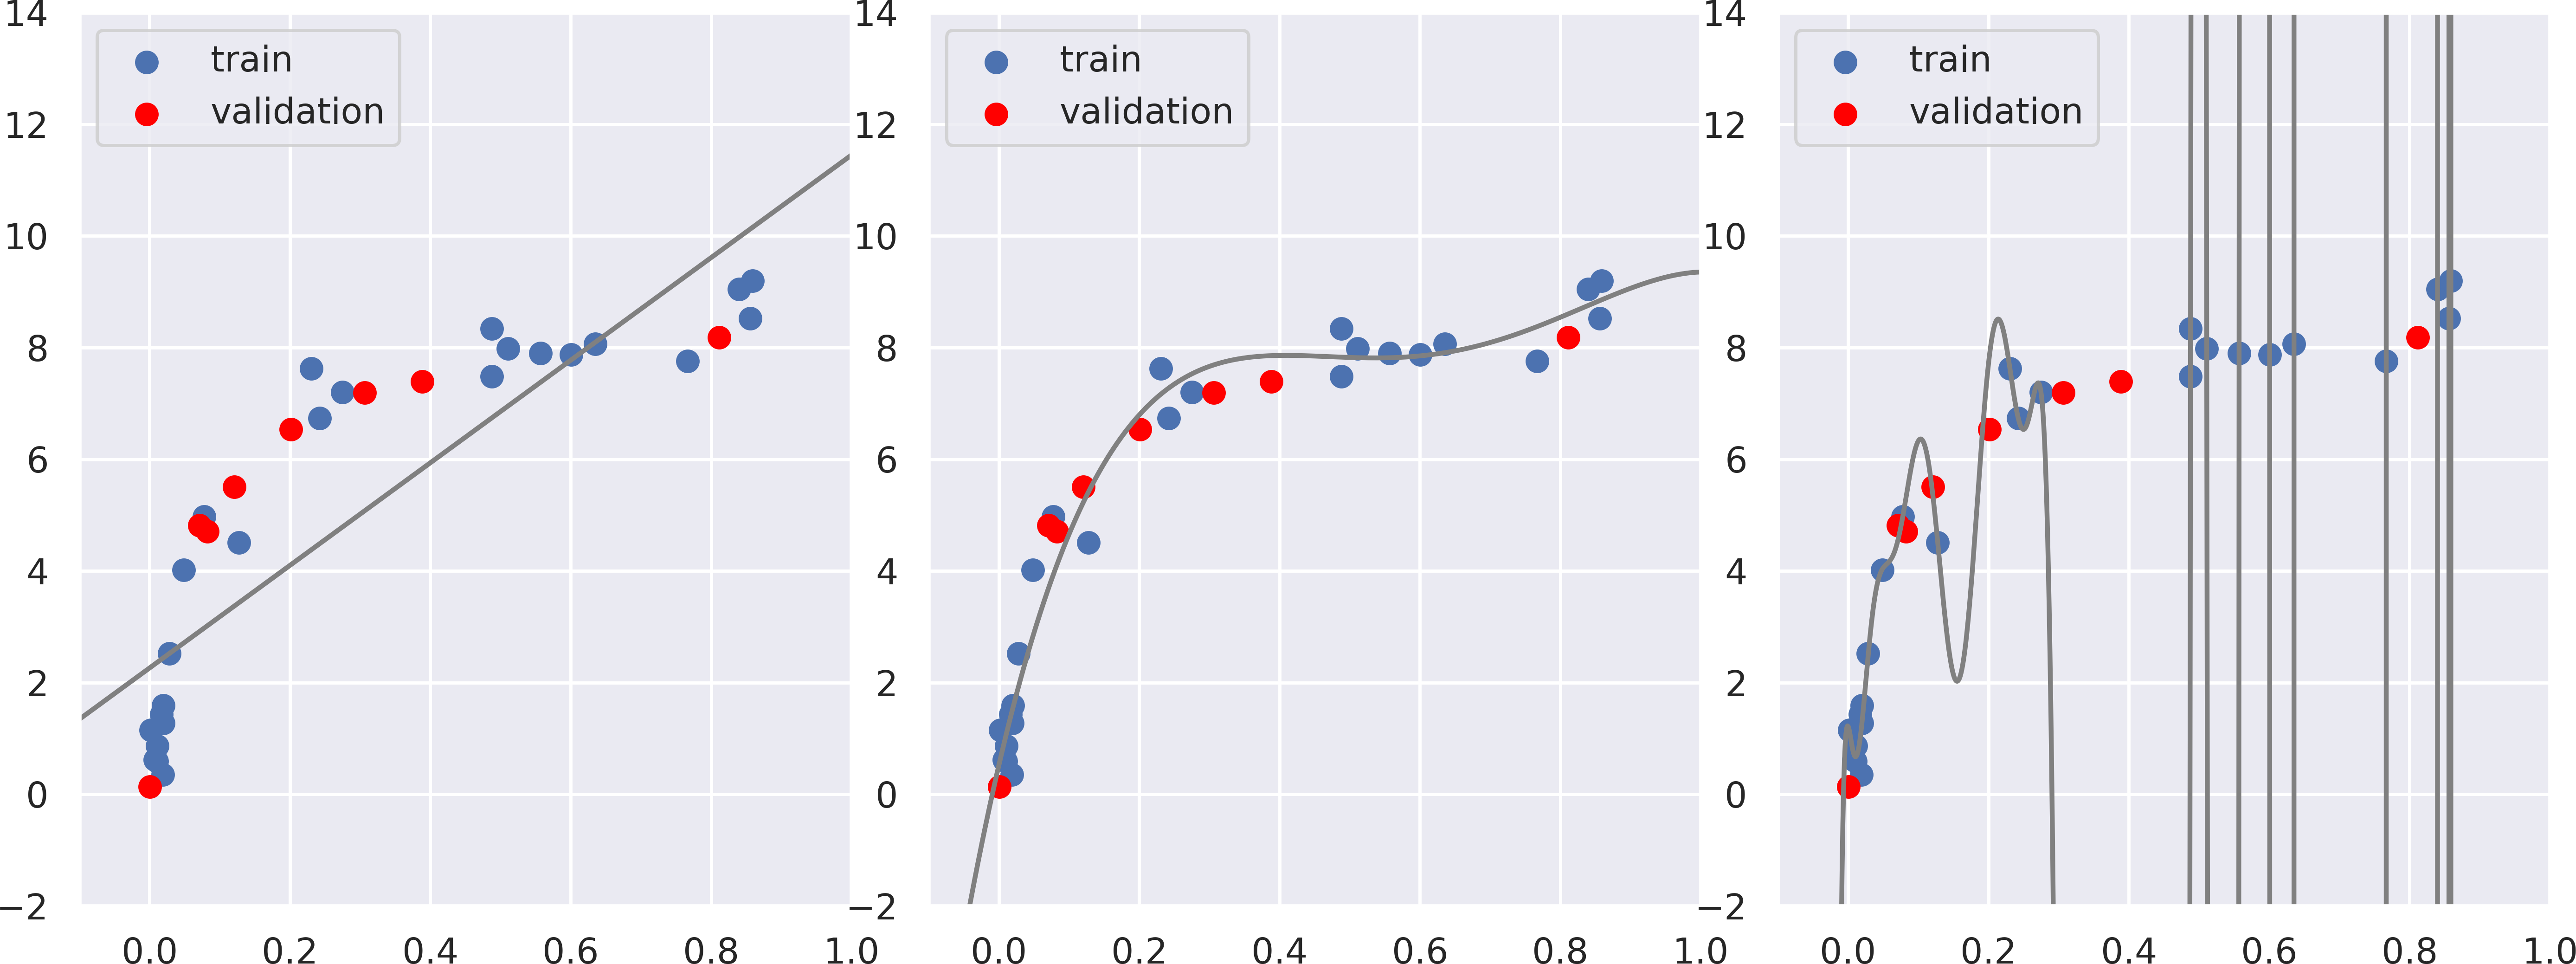
\includegraphics[width=1\textwidth]{overfitting_val}
    \caption{\label{fig:overfitting} A polynomial regression fitted to random data with polynomials of order 1 (left, underfitting), 4 (centre, suitable) and 20 (right, overfitting). Training data is shown in blue, validation data in red. Overfitting leads to better predictions on training data, but poor predictions on validation data (based on \protect\citet{vanderplas_python_2016}).}
\end{figure}

Similarly, in the context of a polynomial regression (Figure \ref{fig:overfitting}), overfitting can be caused by attempting to fit the model using an overly high-order polynomial, while underfitting is caused by using an insufficiently high-order polynomial. \cite[p. 365]{vanderplas_python_2016}

Success in \ac{ml} tasks requires finding a balance between undercomplexity and overcomplexity in the model. To avoid overfitting (or underfitting) on neural networks, a suitable number of training epochs (among other hyperparameters) should be found.

\section{The Engine}
Companies active within civil aerospace companies design and manufactures high-bypass turbofan jet engines, which offer an ideal arrangement for civil aircraft flying below the speed of sound \cite[]{rolls-royce_plc_jet_2015}.

Engines consist of four main components (fan, compressor, combustion chamber and turbine) which correspond approximately to the four stages of a Brayton cycle (intake, compression, combustion, expansion). The engine draws in air, compresses it and burns fuel in the compressed air to further increase the temperature. In this high-pressure, high-temperature state, the air expands and is blown out of the nozzle, driving the turbine on its way which, in turn, powers the fan and compressor and allows the process to continue \cite[]{rolls-royce_plc_jet_2015}.

Many modern civil aircraft engines are equipped with two concentric shafts, split into \ac{lp} and \ac{hp}, which connect respective sets of compressors and turbines \cite[]{spittle_gas_2003}. Some, including the Rolls-Royce Trent family of engines, also have a third shaft, coupling the \ac{ip} compressor and turbine. Figure \ref{fig:triple_spool} shows the configuration of such an engine.

\begin{figure}
    \centering
    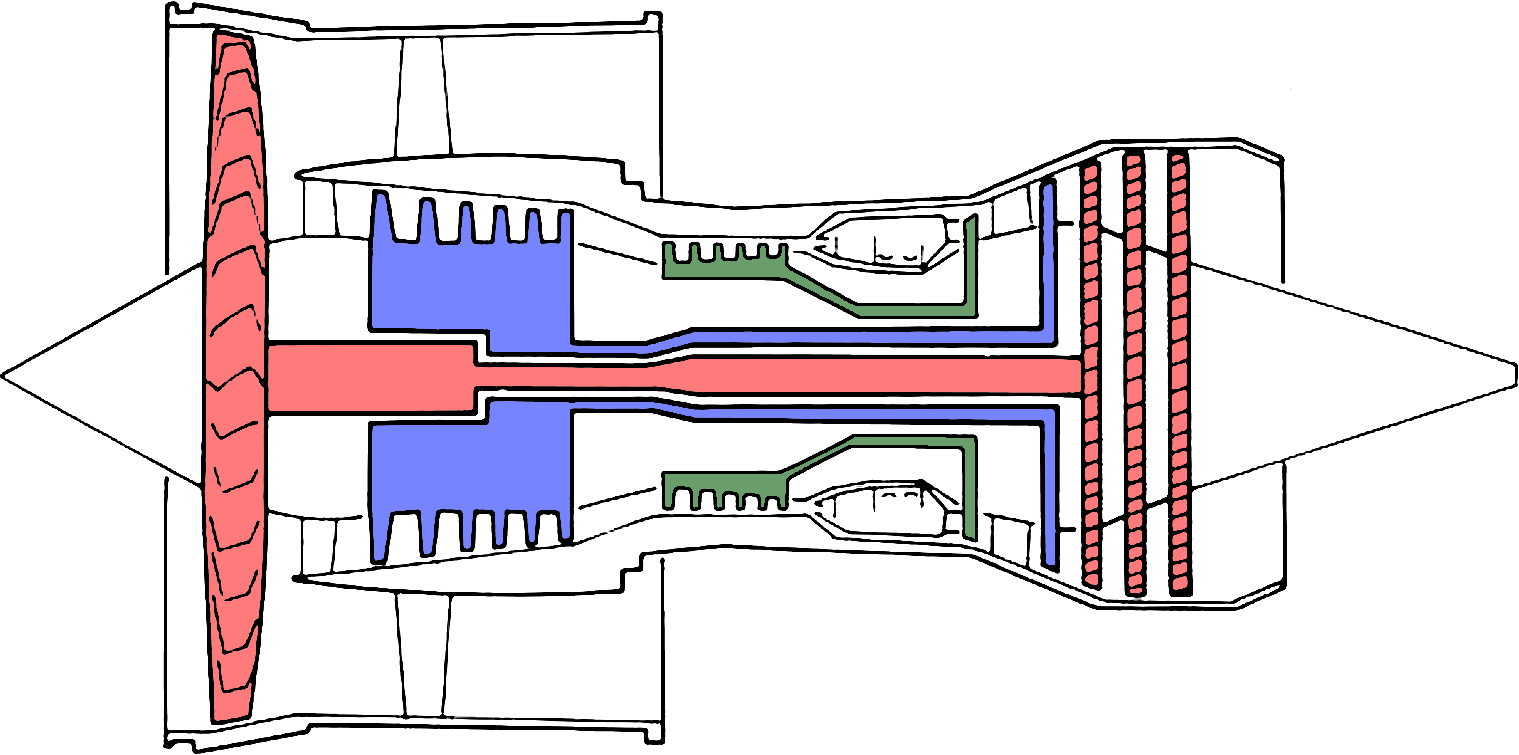
\includegraphics[width=0.7\textwidth]{triple_spool}
    \caption{\label{fig:triple_spool} A schematic diagram of a triple-spool high-bypass engine with \ac{lp}, \ac{ip} and \ac{hp} components shown in red, blue and green, respectively (based on \protect\citet{rolls-royce_plc_jet_2015}).}
\end{figure}

A multi-spool configuration can greatly improve the efficiency of an engine, but comes with some drawbacks. The overall efficiency of an engine, \(\eta_{overall}\), is the product of its thermal and propulsive efficiencies:
\begin{align}
    \eta_{overall} = \eta_{thermal} \cdot \eta_{propulsive}
\end{align}
Assuming an ideal Carnot cycle, the thermal efficiency is given by
\begin{align}
    \eta_{thermal} = 1 - \frac{T_{min}}{T_{max}}
\end{align}
whereby \(T_{min}\) is the engine entry temperature (assumed constant) and \(T_{max}\) the maximum temperature (reached within the combustion chamber). A higher \(T_{max}\) therefore leads to greater thermal efficiency. Increasing the temperature, however, requires %burning more fuel and more oxygen in which to burn the fuel, which in turn necessitates
higher compression. When the engine's overall pressure ratio (the ratio of stagnation pressure between the end and the beginning of the compressor stage) reaches values of 8 to 10, additional shafts become necessary \cite[p. 58]{braunling_flugzeugtriebwerke_2015} in order to enable sufficiently high rotational speeds.

These requirements and developments have led to an average increase in \ac{tet} of 10 K per year over the past 80 years \cite[]{kyprianidis_future_2011}, and in modern engines has reached temperatures far above the melting point of \ac{hpt} blades, requiring great improvements in the materials, structures and systems used \cite[]{spittle_gas_2003}. With this improvement in thermal efficiency, the arrangement comes with the compromise of significantly increased thermomechanical (due to higher temperature) and mechanical loads (due to higher rotational speeds) within the engine, particularly as the air passes from the combustion chamber to the \ac{hpt}.

\section{Damage}\label{damage}
Components used in such extreme conditions experience degradation. They therefore cannot be used indefinitely and must be removed from service after a certain amount of time to avoid potentially catastrophic failure. The amount of time for which the component is permitted for service, referred to as its Approved Life, is determined in safety analyses \cite[]{easa_certification_2015}. Approved Life is measured in Engine Flight Cycles, to be referred to as \textit{cycles} in the following.

The degradation of the engine through its use is referred to as damage. The extent of damage is dependent on many parameters: Since operators use their aircraft for different purposes, flight parameters such as duration, altitude and outside temperature vary greatly and result in different levels of damage. This idea can be quantified with the aforementioned cycles.

In a \ac{fe} context, components are modelled digitally and separated into a finite number of individual elements defined by their corresponding corner points, or nodes. Areas of particular interest within the component (usually where stresses are expected to be highest) are referred to as features.

Within Rolls-Royce, damage from flight missions is currently calculated using one of two internal tools for flight profile analysis: SA66 and Perseus. %(see Sections \ref{sa66} and \ref{pers}, respectively)
The former is ideal for processing many flights in a short amount of time, but is restricted to a low number of features due to the time involved in manually setting up the surrogate \ac{fe} model for each feature. The latter can be described as a brute-force method that determines damage for all surface nodes, but is currently restricted by the amount of time required to process a single flight.

\subsection{Certification}
Certification of a new engine includes a thorough safety analysis as described in \cite{easa_certification_2015}.

Of primary concern is the \ac{hpt} disk due to the extreme conditions under which it operates and the risk of Hazardous Engine Effects. The latter is defined to include (among others) \textquote{non-containment of high-energy debris}, \textquote{uncontrolled fire} and \textquote{complete inability to shut the engine down} according to the \ac{easa} and the \ac{faa} \cite{easa_certification_2015, faa_guidance_2007}. A safety analysis must show that Hazardous Engine Effects are expected to occur with a probability no greater than \(10^{-7}\) per flight hour.

Engine parts whose failure is likely to result in Hazardous Engine Effects are labelled Engine Critical Parts; the \ac{hpt} disk also carries this label. Engine Critical Parts are assigned an Approved Life, which defines the \textquote{mandatory replacement life} \cite{easa_certification_2015} of the part and is measured in Engine Flight Cycles, which are defined by a flight profile that is considered a reference flight mission, corresponding approximately to the average flight for which the engine is expected to be used in service.

Determining a part's Approved Life, commonly referred to as lifing, is a complex process, the majority of which involves \textquote{defining the duty the part is required to sustain} \cite{corran_lifing_2007}, i.e. the design and refinement of the Engine Flight Cycle. One lifing philosophy is that of \ac{ltfc}, which involves determining the \ac{pscl} by means of statistically-determined safety factors.

\subsection{Exchange Rate}
One value calculated from the \ac{ehm} flight data and used as input data for regression models in this thesis is the exchange rate \(ER\). This value is derived from the Palmgren-Miner rule \cite[]{palmgren_lebensdauer_1924} which states that a material will fail when the accumulated damage \(U\), determined by the formula
\begin{align}
    U = \sum_{i}{\frac{n_i}{N_i}},
\end{align}
reaches the value of 1. Here, \(n_i\) is the number of cycles at a certain amplitude \(\sigma_i\) in a stress spectrum \(S\), while \(N_i\) is the number of cycles to failure at \(\sigma_i\) as defined by the material's SN-curve.

The exchange rate is the proportion of \(U\) to the damage from the flight's major cycle, i.e. \(n_{\text{max}} / N_{\text{max}}\) where the subscript \(\text{max}\) denotes the index of the maximum stress amplitude in \(S\). Therefore,
\begin{align}
    ER = \sum_{i}{\frac{n_i}{N_i}} \Big/ {\frac{n_{\text{max}}}{N_{\text{max}}}}.
\end{align}
\section{Research Question} \label{sec:research_q}
Damage as computed by the Cycle Counter or Perseus can be subtracted from the component's Approved Life in order to monitor the remaining life of the component, and remove it from service when this reaches zero. With a view to improving current company processes, this thesis aims to address the following research question:

Using the methods described in this section, can a supervised \ac{ml} or \ac{dl} approach be identified that offers a sufficiently robust, verifiable, comprehensive, scalable, fast and accurate means of processing \ac{ehm} data to determine the extent of damage incurred by surface nodes of a component during real flight missions?

The given input data is \ac{ehm} data from 14\,045 real flight missions (Section \ref{sec:ehm}), coupled with corresponding Cycle Counter damage values (Section \ref{sec:cyclecounter}) for each of the seven features (Section \ref{sec:features}) as the given output data.

Models based on \ac{ml} and \ac{dl} methods will be trained on the complete dataset as well as two subsets (Section \ref{sec:data_sizes}). The aim is to use the trained model to reproduce given output data on unseen input data with the highest possible accuracy. Further, due to the substantial time involved in gathering the given output data, scalability is of great importance. A model is considered scalable if it performs well on a given dataset of minimal length in comparison to a much larger dataset.